\documentclass[12pt,letterpaper]{article}
\usepackage[margin=1in]{geometry}
\usepackage{amsmath,amssymb}
\usepackage{graphicx}
\usepackage[utf8]{inputenc}
\usepackage[T1]{fontenc}
\usepackage{natbib}
\usepackage{setspace}
\usepackage{booktabs}
\usepackage{hyperref}
\usepackage{xcolor}

\hypersetup{colorlinks=true,linkcolor=blue,citecolor=blue,urlcolor=blue}
\doublespacing

\title{The dissolved organic matter clonome: constrained isomeric richness reveals hidden structural diversity across aquatic and terrestrial ecosystems}
\author{[Author~A]$^{1,*}$, [Author~B]$^{1}$, [Author~C]$^{2}$ \\
\small $^1$[Institution] \\
\small $^2$[Institution] \\
\small $^*$Correspondence: [email]}
\date{}

\begin{document}
\maketitle

\begin{abstract}
Each molecular formula detected by Fourier-transform ion cyclotron resonance mass spectrometry (FT-ICR-MS) in dissolved organic matter (DOM) may represent multiple structural isomers with distinct ecological functions---a hidden reservoir we term the `DOM clonome'. Trapped ion mobility spectrometry has confirmed 6--40 isomers per formula, but does not scale to large surveys. We introduce Constrained Isomeric Richness (CIR), a per-formula index that estimates the number of chemically plausible isomers using compound-class--specific structural constraints anchored to published mobility measurements. Applied to 8,972 formulae from 27 river sites in the WHONDRS network and analysed at the site level ($n = 27$), CIR reveals three findings. First, isomeric depth varies systematically by compound class: lipid-like formulae harbour $\sim$19 estimated isomers and aromatic classes $\sim$8. Second, mean CIR of the CRAM fraction shows the strongest correlation with latitude among all tested metrics ($r = -0.79$, $p < 10^{-5}$, $n = 27$), slightly exceeding mean H/C ($r = -0.73$). Third, CIR is negatively correlated with formula richness ($r = -0.40$, $p = 0.039$, $n = 27$), showing that structural depth and compositional breadth are partially decoupled dimensions of DOM complexity. CIR is analytically reproducible (replicate CV $= 0.32\%$) and computationally inexpensive. Applied without modification to six additional datasets spanning river, sediment, soil, Arctic, and marine environments (691,229 total formulae across 1,343 samples), CIR reproduced the same compound class ordering in every case. CRAM isomeric depth followed a gradient consistent with processing intensity: Arctic $<$ sediment $<$ river $<$ soil $<$ marine.
\end{abstract}

\noindent\textbf{Keywords:} dissolved organic matter, FT-ICR-MS, isomeric richness, WHONDRS, DOM clonome, chemodiversity, CRAM

\section{Introduction}

\subsection{The DOM clonome and the isomeric blind spot}

Dissolved organic matter (DOM) fuels aquatic biogeochemistry, yet its true structural complexity remains largely invisible. Ultrahigh-resolution mass spectrometry (FT-ICR-MS) has transformed our understanding of DOM by resolving it into thousands of distinct molecular formulae \citep{stenson2003,kujawinski2002}. However, this view is fundamentally incomplete because FT-ICR-MS detects exact masses, not structural architectures. Each formula may correspond to multiple constitutional isomers---molecules sharing atomic composition but differing in bond connectivity, ring configuration, and functional group placement. These structural differences matter: isomers of a given formula can differ in biodegradability \citep{ohno2014}, photoreactivity \citep{stubbins2010}, and metal-binding capacity \citep{aiken2011}.

Trapped ion mobility spectrometry coupled to FT-ICR-MS (TIMS-FT-ICR-MS) has made this hidden diversity directly observable. \citet{leyva2019,leyva2020} showed that individual DOM formulae resolve into 6--40 mobility-separated peaks, each representing a structurally different isomer. By analogy to immunology---where a single phenotypic marker hides a diverse repertoire of T cell clones \citep{qi2014}---we conceptualise this hidden structural reservoir as the `DOM clonome'. However, TIMS requires specialised instrumentation available in very few laboratories, making it impractical for large-scale environmental surveys.

\subsection{Estimating Constrained Isomeric Richness}

Full constitutional isomer enumeration is computationally intractable for DOM-sized molecules \citep{benecke1997}, but most theoretical isomers are chemically implausible in natural waters. DOM derives from a limited set of biosynthetic precursors---lignin, terpenoids, proteins, carbohydrates \citep{dittmar2014}---and aquatic chemistry imposes additional constraints. We introduce Constrained Isomeric Richness (CIR), a heuristic index that estimates the size of the chemically plausible isomer subset by scoring structural degrees of freedom after applying compound-class--specific constraints. The penalty structure reflects fundamental chemical expectations: carbohydrate-like formulae are expected to have fewer plausible constitutional arrangements than lipid-like formulae, because extensive oxygenation and required ring formations constrain the space of viable structures. CIR translates these expectations into a quantifiable, per-formula metric of structural depth, anchored to the TIMS-observed range.

\subsection{Study objectives}

We applied CIR to 8,972 formulae across 80 replicate samples (27 sites) from the WHONDRS 2018 surface water campaign \citep{stegen2022,goldman2020}, with all environmental correlations computed at the site level ($n = 27$) to avoid pseudoreplication. We then tested cross-ecosystem portability by applying the same pipeline, without parameter adjustment, to WHONDRS Summer 2019 sediment porewater (127,136 formulae from 276 samples), WHONDRS Summer 2019 surface water (166,262 formulae from 282 samples at 97 global sites), WHONDRS WROL 2019 watershed resilience campaign (150,999 formulae, 501 samples), Yukon Delta Experiment 2021 Arctic sediment (86,338 formulae, 180 samples), soil DOM from a Chinese paddy field fertilisation experiment (121,324 formulae, 21 samples; \citealt{xia2025}), and marine DOM from the Weddell Sea and North Sea (30,198 formulae; \citealt{moye2025}). We tested whether: (1) CIR varies among compound classes consistently with structural chemistry across ecosystem types; (2) CIR correlates with environmental gradients more strongly than simpler metrics; and (3) CIR is partially independent of conventional formula richness.

\section{Methods}

\subsection{Study system}

Surface water triplicate samples from 27 river sites across eight U.S. states (30.2$^\circ$--46.4$^\circ$N; WHONDRS 2018 campaign; \citealt{stegen2022}; \citealt{goldman2020}). Water temperature: 6--63$^\circ$C (the 63$^\circ$C site is likely geothermally influenced; excluding it did not alter results). DOC: 0.9--5.2~mg~L$^{-1}$.

\subsection{FT-ICR-MS}

12-Tesla FT-ICR-MS at the Environmental Molecular Sciences Laboratory \citep{tfaily2015}. Formula constraints: C$_{1\text{--}57}$H$_{1\text{--}100}$O$_{0\text{--}30}$N$_{0\text{--}5}$S$_{0\text{--}3}$P$_{0\text{--}2}$; mass error $< 1$~ppm \citep{koch2007}. Of 34,021 features, 8,972 received assignments.

\subsection{Compound class assignment}

Indices: DBE $= 1 + \text{C} - \text{H}/2 + \text{N}/2$; AI$_\text{mod}$ \citep{koch2006}; NOSC \citep{larowe2011}. Classes assigned in priority order: (1) condensed aromatic (AI$_\text{mod} \geq 0.66$); (2) aromatic ($0.50 \leq \text{AI}_\text{mod} < 0.66$); (3) CRAM (H/C $< 1.5$, O/C $< 0.5$; \citealt{hertkorn2006}); (4) carbohydrate-like (H/C $\geq 1.5$, O/C $\geq 0.5$); (5) lipid-like (H/C $\geq 1.5$, O/C $< 0.5$); (6) protein-like (N $> 0$, H/C $> 1.3$); (7) N-containing (N $> 0$); (8) unclassified.

\subsection{CIR scoring function}

The complete CIR equation:
\begin{align}
\log_{10}(\text{CIR})_\text{raw} &= 0.8 \cdot \log_{10}(\max(1, \text{C}-3)) \nonumber \\
&+ \max(0.1,\; -0.15(\text{DBE}-4)^2 + 1.2) \nonumber \\
&+ w_\text{O} \cdot \log_{10}(\max(1, \text{O})) \nonumber \\
&+ 0.5 \cdot \log_{10}(\max(1, \text{N}+1)) \nonumber \\
&- 0.12 \cdot n_\text{req} - 0.05 \cdot n_\text{forb} - P_\text{arom} - P_\text{ring}
\end{align}
where $w_\text{O} = 0.4$ for carbohydrate-like, 0.7 otherwise; $P_\text{arom} = \text{AI}_\text{mod} \times 0.8$ for aromatic classes (0 otherwise); $P_\text{ring} = \max(0, \text{DBE} - R_\text{max}) \times 0.1$. Chemically disfavoured features (peroxide bonds, triple bonds, 3- and 4-membered rings) were not explicitly enumerated; instead, their implausibility was encoded as score penalties ($n_\text{forb}$). The raw score was rescaled:
\begin{equation}
\log_{10}(\text{CIR}) = 0.78 + \frac{\log_{10}(\text{CIR})_\text{raw}}{3.0} \times 0.82, \quad \text{clipped to } [0.3, 1.70]
\end{equation}
The lower anchor (0.78) corresponds to $\log_{10}(6)$; the scaling factor (0.82) maps a normalised raw-score range onto an upper value near 1.60 ($\approx \log_{10}(40)$), matching the TIMS-observed range \citep{leyva2019}. The upper clip (1.70) adds headroom; in practice no formula exceeded 1.58.

\subsection{Aggregation and statistics}

Formula-level CIR was aggregated as intensity-weighted mean $\log_{10}$(\text{CIR}) per sample \citep{tfaily2015}, then averaged across triplicates to yield site-level means. All environmental correlations are reported at the site level ($n = 27$). Monte Carlo sensitivity analysis (500 iterations, all coefficients perturbed $\pm 10\%$) confirmed robustness (Supplementary Methods S4.4). The pipeline (Python 3.12, 306 lines, open-source) runs in $\sim$2~s.

\section{Results}

\subsection{Compound classes and formula-level CIR}

CIR varied systematically across compound classes (Figure~\ref{fig:main}A; Table~\ref{tab:classes}). Aromatic classes exhibited the lowest median CIR ($\sim$8 estimated isomers), and lipid-like formulae the highest ($\sim$19). CRAM was intermediate ($\sim$10). The CIR range (0.30--1.58) was anchored to the TIMS-observed range of 6--40 isomers \citep{leyva2019}; no assigned formulae produced undefined values.

\begin{table}[ht]
\centering
\caption{Formula-level CIR by compound class ($\log_{10}$ scale), ordered by median.}
\label{tab:classes}
\begin{tabular}{lrrrrr}
\toprule
Compound class & $n$ & Mean & SD & Median & $\sim$Isomers \\
\midrule
Aromatic & 1,136 & 0.876 & 0.055 & 0.881 & 7.6 \\
Condensed aromatic & 446 & 0.883 & 0.088 & 0.896 & 7.9 \\
CRAM & 2,735 & 0.998 & 0.090 & 0.988 & 9.7 \\
Protein-like & 205 & 1.124 & 0.090 & 1.086 & 12.2 \\
Carbohydrate-like & 951 & 1.173 & 0.113 & 1.199 & 15.8 \\
N-containing & 472 & 1.231 & 0.042 & 1.237 & 17.3 \\
Unclassified & 1,802 & 1.257 & 0.061 & 1.252 & 17.8 \\
Lipid-like & 1,225 & 1.260 & 0.126 & 1.267 & 18.5 \\
\midrule
\textbf{Total} & \textbf{8,972} & & & & \\
\bottomrule
\end{tabular}
\end{table}

\subsection{Site-level environmental correlations}

CIR of the CRAM fraction (CIR$_\text{CRAM}$) showed the strongest environmental signal (Table~\ref{tab:correlations}). The site-level latitude correlation ($r = -0.79$, $p < 10^{-5}$) was the strongest among the tested summary metrics, including mean H/C of the CRAM fraction ($r = -0.73$), mean DBE ($r = 0.71$), and mean molecular weight ($r = 0.67$; Table~\ref{tab:comparison}). The margin over mean H/C is modest ($|\Delta r| = 0.06$). Leave-one-site-out cross-validation yielded $r$ values between $-0.73$ and $-0.83$. Bulk mean CIR correlated with latitude ($r = -0.40$, $p = 0.040$) but not significantly with temperature ($r = 0.27$, $p = 0.17$) at the site level.

\begin{table}[ht]
\centering
\caption{Correlations between CIR and environmental variables at the site level ($n = 27$).}
\label{tab:correlations}
\begin{tabular}{llrr}
\toprule
Variable & CIR metric & $r$ & $p$ \\
\midrule
Latitude & Mean CIR & $-0.397$ & 0.040 \\
Temperature & Mean CIR & 0.271 & 0.17 \\
DOC & Mean CIR & 0.111 & 0.58 \\
Formula richness & Mean CIR & $-0.400$ & 0.039 \\
Latitude & CIR$_\text{CRAM}$ & $\mathbf{-0.785}$ & $\mathbf{<10^{-5}}$ \\
Temperature & CIR$_\text{CRAM}$ & $\mathbf{0.631}$ & $\mathbf{<0.001}$ \\
DOC & CIR$_\text{CRAM}$ & $\mathbf{0.426}$ & $\mathbf{0.027}$ \\
\bottomrule
\end{tabular}
\end{table}

\begin{table}[ht]
\centering
\caption{CIR$_\text{CRAM}$ vs.\ simpler CRAM-fraction metrics for latitude prediction ($n = 27$).}
\label{tab:comparison}
\begin{tabular}{lrr}
\toprule
Metric & $|r|$ vs.\ latitude & $p$ \\
\midrule
\textbf{CIR$_\text{CRAM}$} & \textbf{0.785} & $<10^{-5}$ \\
Mean H/C (CRAM) & 0.726 & $<10^{-4}$ \\
Mean DBE (CRAM) & 0.711 & $<10^{-4}$ \\
Mean mass (CRAM) & 0.667 & $<10^{-3}$ \\
Mean AI$_\text{mod}$ (CRAM) & 0.643 & $<10^{-3}$ \\
\bottomrule
\end{tabular}
\end{table}

\subsection{Independence from formula richness}

Site-level mean CIR and formula richness were negatively correlated ($r = -0.40$, $p = 0.039$, $n = 27$). Restricting to formulae present in all three replicates per site (reducing mean formulae from 2,245 to 1,592), recomputing site-level means, and retesting yielded $r = -0.42$ ($p = 0.030$, $n = 27$). The partial decoupling of structural depth and compositional breadth is a genuine ecological pattern, not an artefact of detection sensitivity.

\subsection{Replicate precision}

Mean CV of CIR across triplicates: 0.32\% (27 sites).

\subsection{Cross-ecosystem application}

We applied the same pipeline without parameter adjustment to six additional FT-ICR-MS datasets (Table~\ref{tab:crosseco}). The compound class ordering was conserved across all seven datasets: aromatic classes occupied the low end and lipid-like formulae the high end in every case. CRAM isomeric depth followed a gradient from Arctic sediment (0.942; $\sim$9 isomers) through temperate river surface water and sediment porewater (0.951--0.988) to soil (1.015; $\sim$10) and marine DOM (1.023; $\sim$11). Arctic DOM (Yukon Delta) had the lowest CRAM CIR, consistent with cold-temperature-limited degradation pathways. Soil DOM showed the highest lipid-like CIR (1.327) of any dataset. Marine DOM was overwhelmingly CRAM (48\%), consistent with the known dominance of refractory CRAM in ocean dissolved organic carbon \citep{hertkorn2006}.

\begin{table}[ht]
\centering
\caption{CRAM median $\log_{10}$(CIR) across seven datasets, ordered by isomeric depth.}
\label{tab:crosseco}
\begin{tabular}{lrlrr}
\toprule
Dataset & Formulae & Type & CRAM med. & $\sim$Iso. \\
\midrule
WHONDRS YDE21 (Arctic) & 86,338 & Arctic sediment & 0.942 & 8.7 \\
WHONDRS S19S Sediment & 127,136 & Sediment porewater & 0.951 & 8.9 \\
WHONDRS S19S Surface Water & 166,262 & River surface (97 sites) & 0.956 & 9.0 \\
WHONDRS WROL 2019 & 150,999 & Watershed resilience & 0.956 & 9.0 \\
WHONDRS 2018 Surface Water & 8,972 & River surface (27 sites) & 0.988 & 9.7 \\
Soil DOM (Xia \& Liu 2025) & 121,324 & Paddy soil & 1.015 & 10.4 \\
Marine DOM (Moye et al.\ 2025) & 30,198 & Marine water column & 1.023 & 10.5 \\
\midrule
\textbf{Total} & \textbf{691,229} & & & \\
\bottomrule
\end{tabular}
\end{table}

\begin{figure}[ht]
\centering
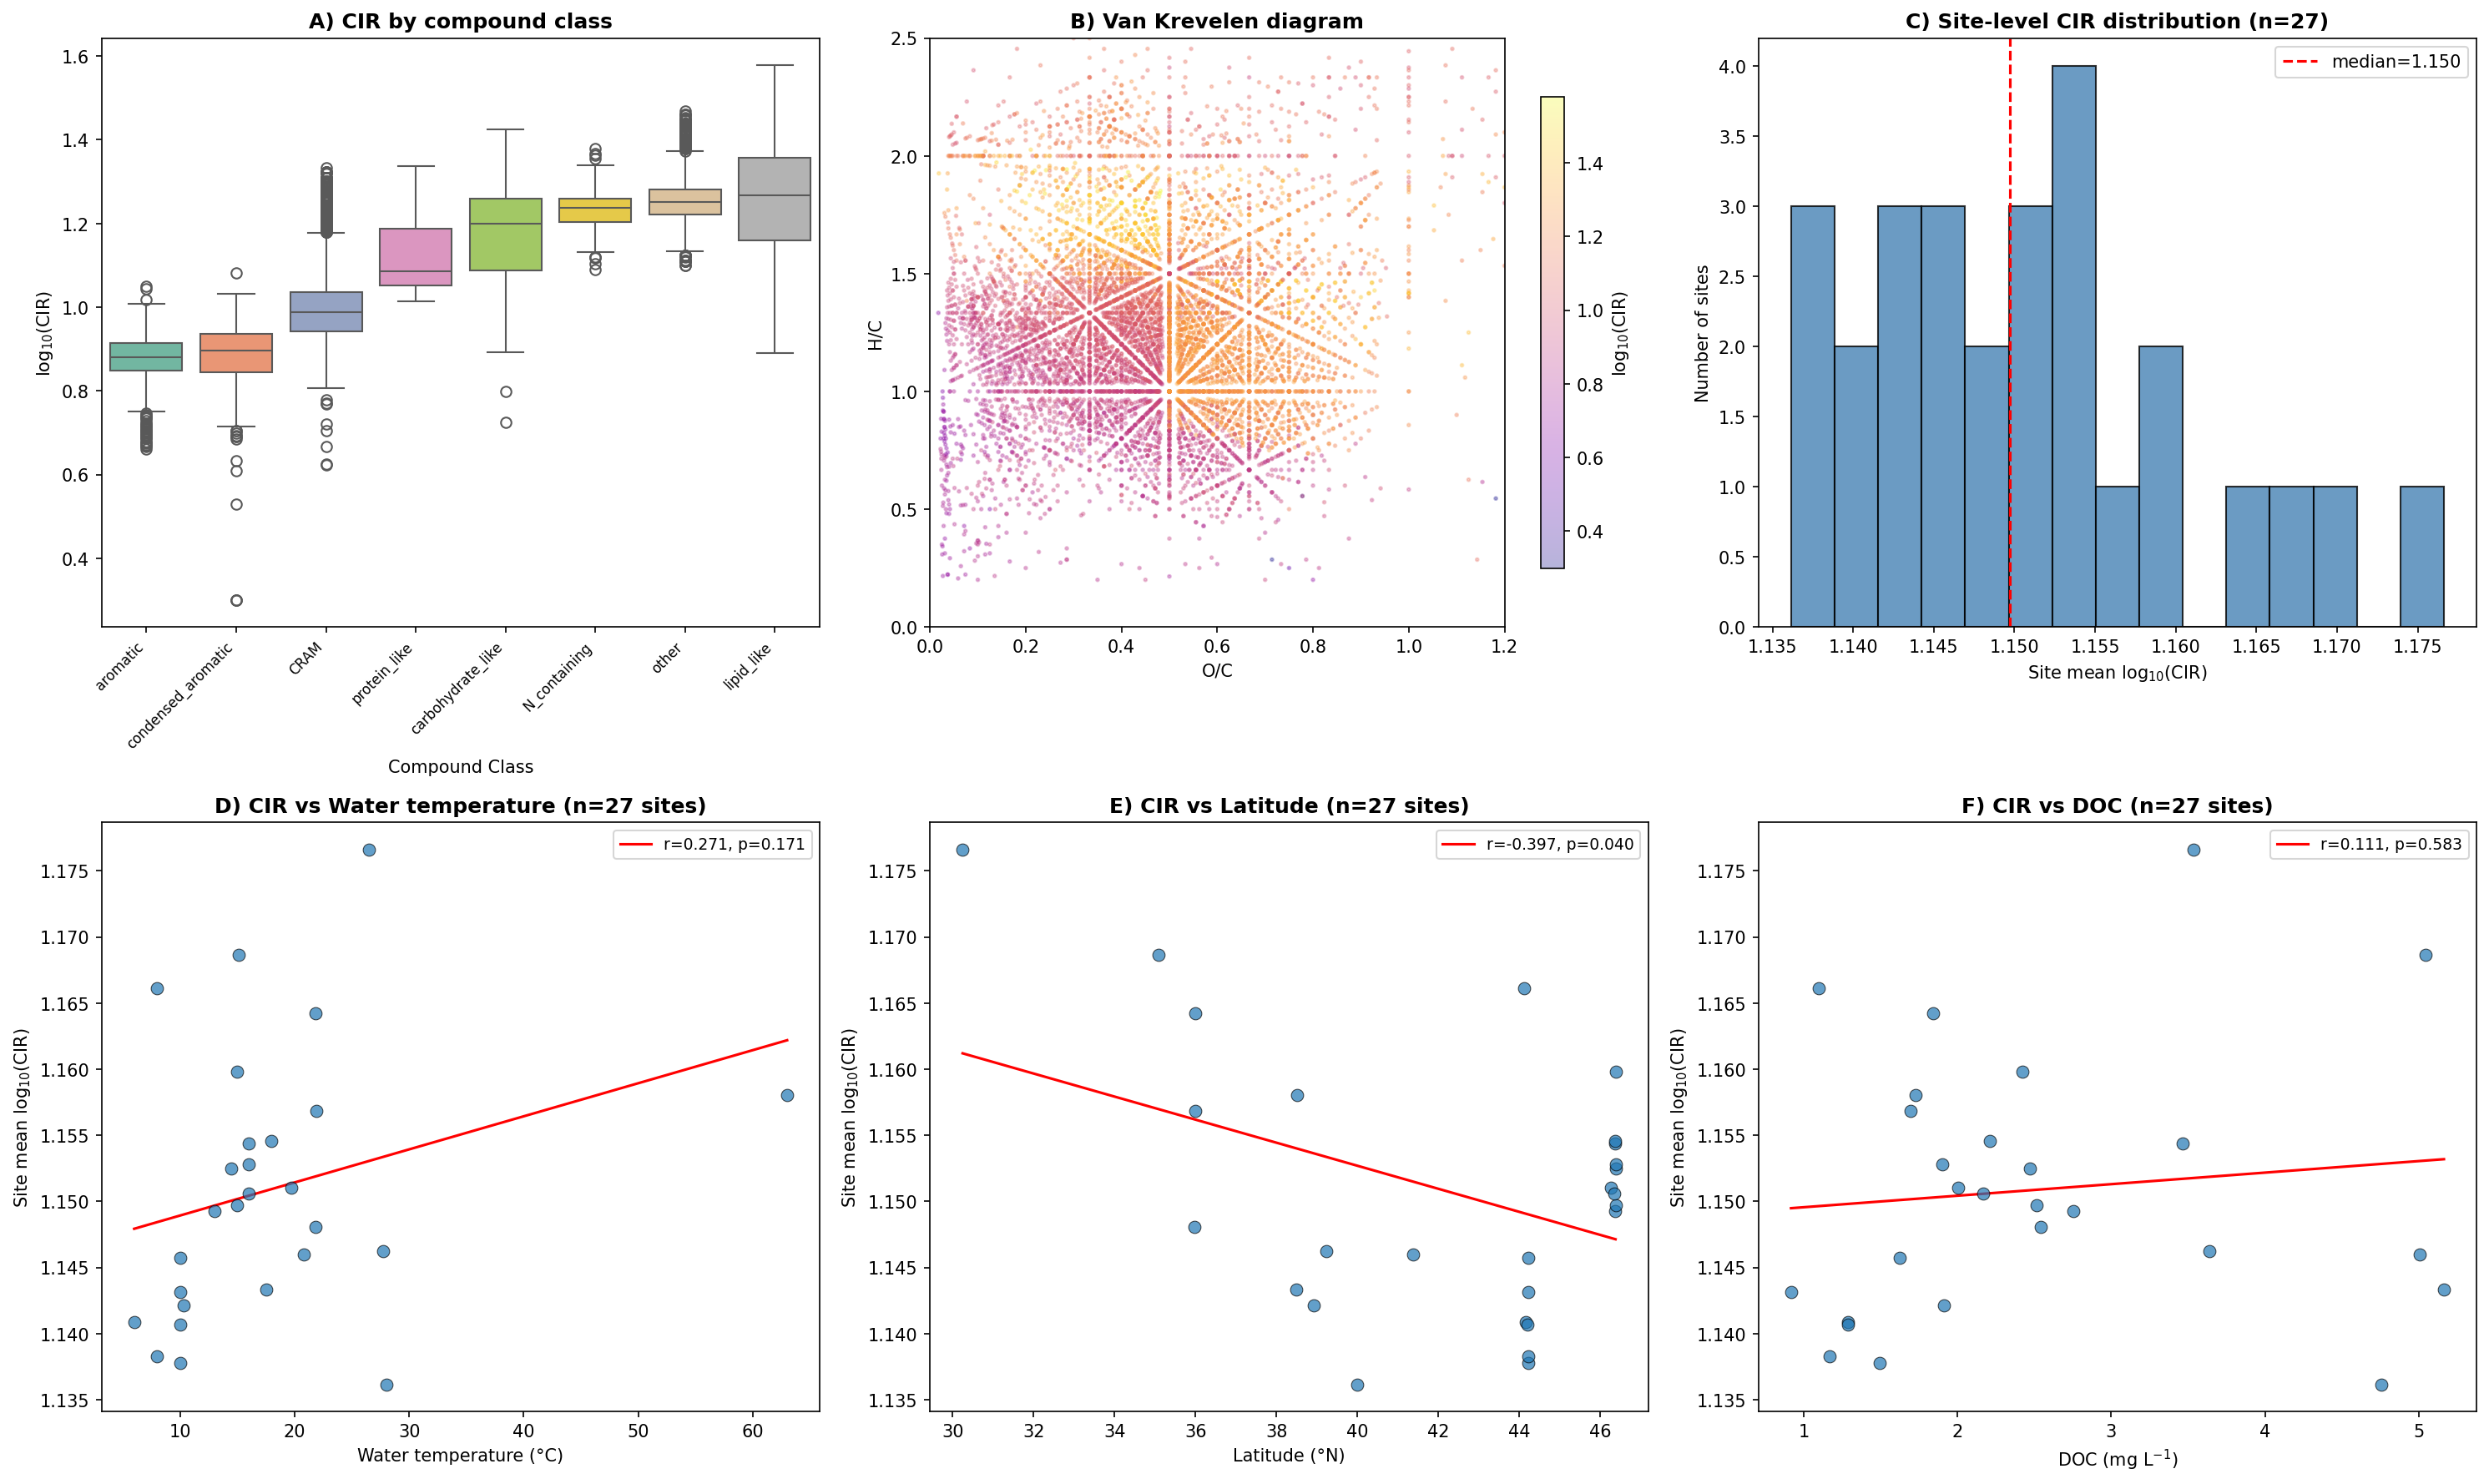
\includegraphics[width=\textwidth]{CIR_results.png}
\caption{CIR across 27 WHONDRS river sites. (A) CIR by compound class (formula level). (B) Van Krevelen diagram coloured by CIR. (C) Site-level CIR distribution ($n = 27$ site means). (D--F) Site mean CIR vs.\ temperature, latitude, and DOC; each point is one site (triplicate mean); regression lines fitted to site means.}
\label{fig:main}
\end{figure}

\begin{figure}[ht]
\centering
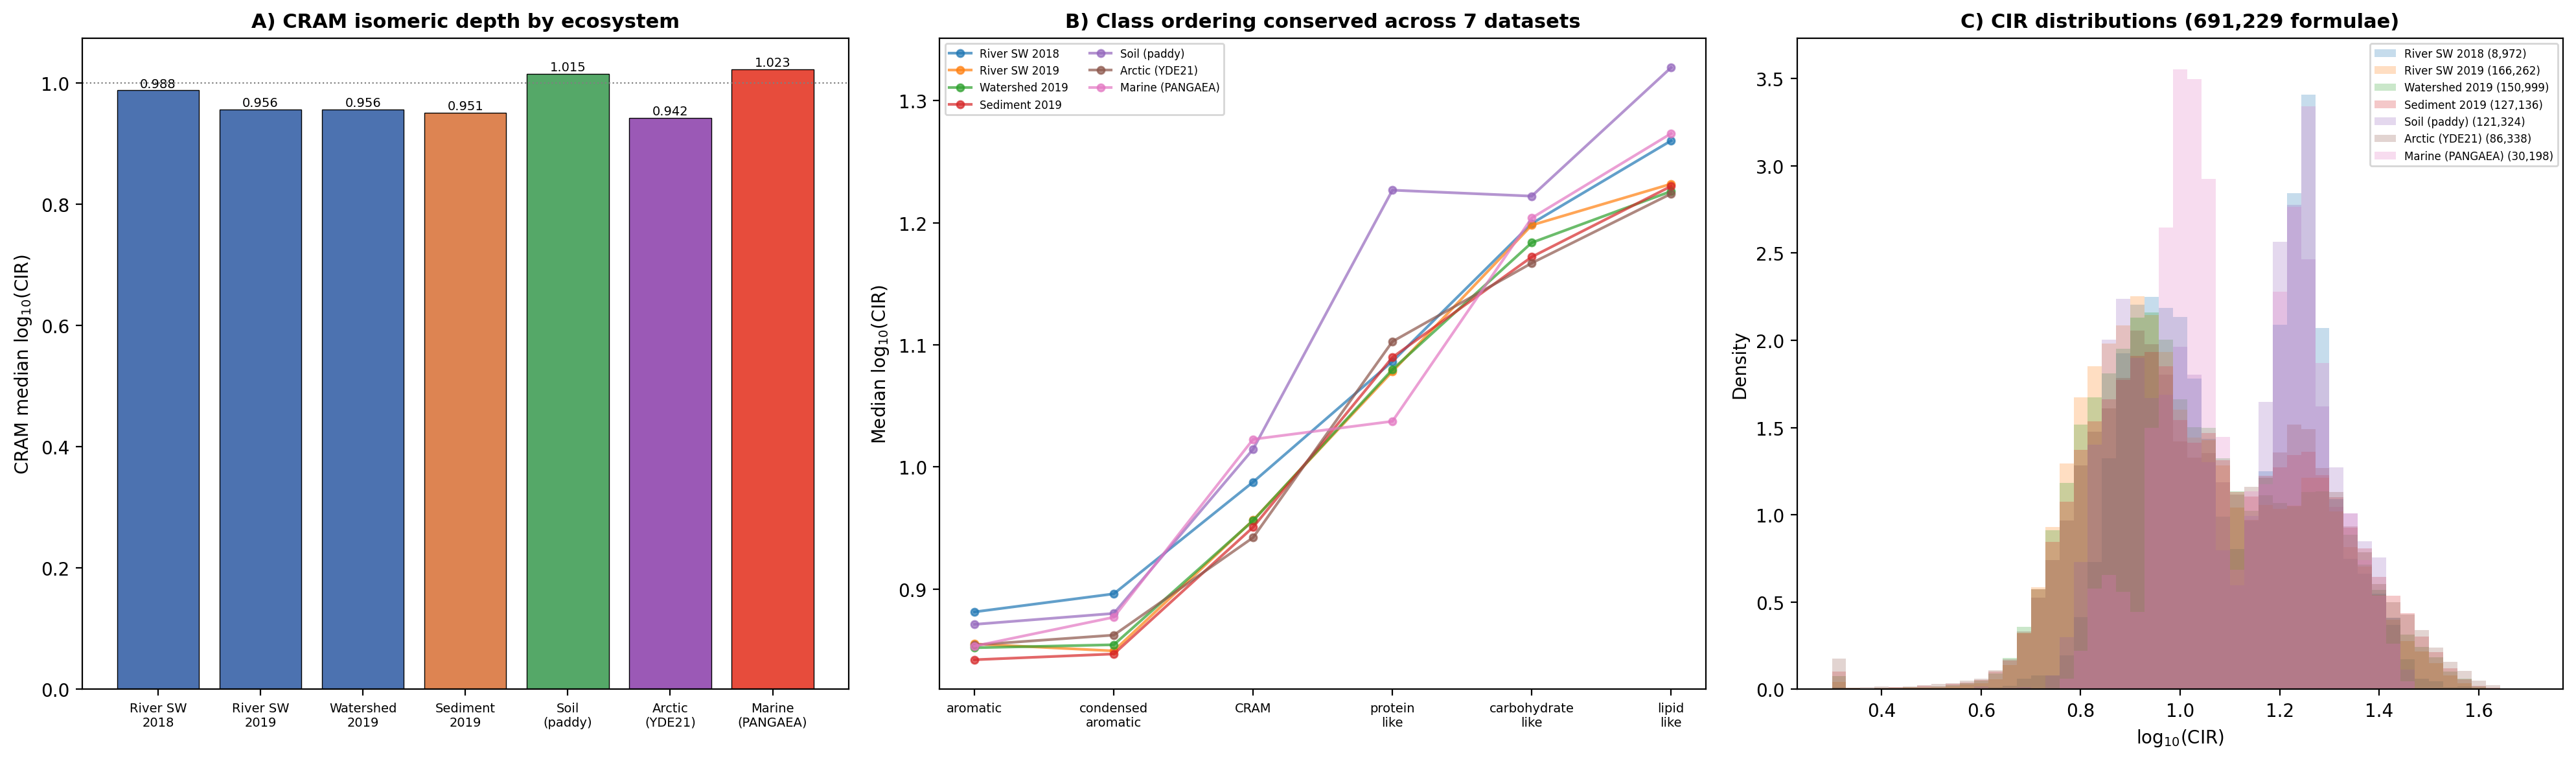
\includegraphics[width=\textwidth]{CIR_cross_ecosystem.png}
\caption{Cross-ecosystem CIR comparison across seven datasets (691,229 formulae). (A) CRAM median CIR by dataset. Blue: river/watershed; orange: sediment; green: soil; purple: Arctic; red: marine. (B) Class ordering reproduced across all seven datasets. (C) CIR density distributions.}
\label{fig:crosseco}
\end{figure}

\section{Discussion}

\subsection{Chemical coherence of the class ordering}

CIR orders compound classes in a manner broadly consistent with structural organic chemistry: flexible aliphatic chains (lipid-like) score highest, rigid fused ring systems (aromatics) score lowest, and alicyclic CRAM is intermediate. Under a null-penalty model (uniform constraints), the rank ordering shifts---indicating that class-specific penalties modulate magnitude. However, the key results (CRAM latitudinal gradient, CIR--richness dissociation) are driven by \emph{within-class} variation and are not sensitive to between-class ranking.

\subsection{The CRAM isomeric gradient}

The site-level CIR$_\text{CRAM}$--latitude correlation ($r = -0.79$) is the strongest among the tested summary metrics, though the margin over mean H/C is modest ($|\Delta r| = 0.06$). Monte Carlo sensitivity analysis (500 iterations, all coefficients $\pm 10\%$) yielded a mean $r = -0.68$ [95\% CI: $-0.69$, $-0.67$], with 100\% of iterations significant at $p < 0.001$. A plausible mechanism is that higher temperatures expand kinetically accessible degradation pathways \citep{larowe2011}, generating more structurally diverse CRAM products. Leave-one-site-out cross-validation yielded $r \in [-0.83, -0.73]$.

\subsection{Breadth versus depth}

The negative site-level CIR--richness correlation ($r = -0.40$, $p = 0.039$), confirmed after replicate filtering ($r = -0.42$, $p = 0.030$), indicates that structural depth within formulae and compositional breadth across formulae are partially decoupled dimensions of DOM molecular complexity. This parallels the distinction between species richness and functional diversity in ecology \citep{petchey2006}.

\subsection{Cross-ecosystem coherence}

The conservation of class ordering across all seven datasets provides the strongest evidence that CIR reflects underlying structural chemistry rather than dataset-specific artefacts. The CRAM isomeric depth gradient (Arctic $<$ sediment $<$ river $<$ soil $<$ marine) is broadly consistent with a processing-intensity hypothesis. Arctic DOM, subject to cold temperatures that limit degradation pathways, shows the lowest CRAM CIR. Marine DOM, processed for years to millennia \citep{dittmar2014}, shows the highest.

\subsection{Practical value and limitations}

CIR requires no new measurements and runs in $\sim$2~s. We demonstrated portability across seven independent datasets totalling 691,229 formulae from river, sediment, soil, Arctic, and marine environments. CIR is a heuristic index. The constraint rules encode current knowledge. Paired TIMS--FT-ICR-MS validation is the critical next step.

\section{Conclusions}

CIR is a heuristic, formula-based estimate of chemically plausible isomeric depth. Applied to the WHONDRS network with properly non-pseudoreplicated statistics ($n = 27$), the isomeric richness of CRAM tracks latitude at $r = -0.79$---the strongest among the tested summary metrics---and structural depth and compositional breadth are partially decoupled axes of DOM complexity. Cross-ecosystem application to seven datasets spanning 691,229 formulae confirmed the class ordering without parameter adjustment and revealed a CRAM isomeric depth gradient (Arctic $<$ sediment $<$ river $<$ soil $<$ marine) consistent with processing intensity. CIR is computationally inexpensive, reproducible, and applicable to the large archive of existing FT-ICR-MS datasets.

\section*{Acknowledgments}
WHONDRS data: ESS-DIVE. Marine DOM: PANGAEA (Moye et al.\ 2025). Soil DOM: Dryad (Xia \& Liu 2025). FT-ICR-MS: EMSL, PNNL.

\section*{Data availability}
WHONDRS: ESS-DIVE. PANGAEA: doi:10.1594/PANGAEA.974714. Dryad: doi:10.5061/dryad.pvmcvdnw4. Code: \url{https://github.com/erikafreeman/dom-clonome}.

\bibliographystyle{apalike}
\begin{thebibliography}{99}

\bibitem[Aiken et al., 2011]{aiken2011}
Aiken, G.R., Hsu-Kim, H., Ryan, J.N. (2011).
Influence of dissolved organic matter on the environmental fate of metals, nanoparticles, and colloids.
\textit{Environ. Sci. Technol.}, 45, 3196--3201.

\bibitem[Benecke et al., 1997]{benecke1997}
Benecke, C., Grund, R., Hohberger, R., Kerber, A., Laue, R., Wieland, T. (1997).
MOLGEN+, a generator of connectivity isomers and stereoisomers.
\textit{Anal. Chim. Acta}, 314, 141--147.

\bibitem[Danczak et al., 2020]{danczak2020}
Danczak, R.E., Goldman, A.E., Chu, R.K., et al. (2020).
Using metacommunity ecology to understand environmental metabolomes.
\textit{Nat. Commun.}, 11, 6369.

\bibitem[Dittmar and Stubbins, 2014]{dittmar2014}
Dittmar, T., Stubbins, A. (2014).
Dissolved organic matter in aquatic systems.
In: \textit{Treatise on Geochemistry}, 2nd ed., v. 12, pp. 125--156. Elsevier.

\bibitem[Goldman et al., 2020]{goldman2020}
Goldman, A.E., Graham, E.B., Crump, A.R., et al. (2020).
Biogeochemical cycling at the aquatic--terrestrial interface.
\textit{Biogeosciences}, 17, 3685--3700.

\bibitem[Hertkorn et al., 2006]{hertkorn2006}
Hertkorn, N., Benner, R., Frommberger, M., et al. (2006).
Characterization of a major refractory component of marine dissolved organic matter.
\textit{Geochim. Cosmochim. Acta}, 70, 2990--3010.

\bibitem[Kim et al., 2003]{kim2003}
Kim, S., Kramer, R.W., Hatcher, P.G. (2003).
Graphical method for analysis of ultrahigh-resolution broadband mass spectra of natural organic matter.
\textit{Anal. Chem.}, 75, 5336--5344.

\bibitem[Koch and Dittmar, 2006]{koch2006}
Koch, B.P., Dittmar, T. (2006).
From mass to structure: an aromaticity index for high-resolution mass data of natural organic matter.
\textit{Rapid Commun. Mass Spectrom.}, 20, 926--932.

\bibitem[Koch et al., 2007]{koch2007}
Koch, B.P., Dittmar, T., Witt, M., Kattner, G. (2007).
Fundamentals of molecular formula assignment to ultrahigh resolution mass data of natural organic matter.
\textit{Anal. Chem.}, 79, 1758--1763.

\bibitem[Kujawinski, 2002]{kujawinski2002}
Kujawinski, E.B. (2002).
ESI FT-ICR MS: characterization of complex environmental mixtures.
\textit{Environ. Forensics}, 3, 207--216.

\bibitem[LaRowe and Van Cappellen, 2011]{larowe2011}
LaRowe, D.E., Van Cappellen, P. (2011).
Degradation of natural organic matter: a thermodynamic analysis.
\textit{Geochim. Cosmochim. Acta}, 75, 2030--2042.

\bibitem[Leyva et al., 2019]{leyva2019}
Leyva, D., Tose, L.V., Porter, J., Wolber, J., Schrader, R., Fernandez-Lima, F. (2019).
Understanding the structural complexity of dissolved organic matter: isomeric diversity.
\textit{Faraday Discuss.}, 218, 431--440.

\bibitem[Leyva et al., 2020]{leyva2020}
Leyva, D., Jaffe, R., Fernandez-Lima, F. (2020).
Structural characterization of DOM using TIMS-FT-ICR MS/MS.
\textit{Anal. Chem.}, 92, 11960--11966.

\bibitem[Moye et al., 2025]{moye2025}
Moye, F., Bareth, M., Koch, B.P., Tebben, J., Harder, T. (2025).
Marine DOM molecular composition by online LC-FT-ICR-MS [dataset]. PANGAEA.

\bibitem[Ohno et al., 2014]{ohno2014}
Ohno, T., Parr, T.B., Gruselle, M.-C.I., et al. (2014).
Molecular composition and biodegradability of soil dissolved organic matter.
\textit{Environ. Sci. Technol.}, 48, 7229--7236.

\bibitem[Petchey and Gaston, 2006]{petchey2006}
Petchey, O.L., Gaston, K.J. (2006).
Functional diversity: back to basics and looking forward.
\textit{Ecol. Lett.}, 9, 741--758.

\bibitem[Qi et al., 2014]{qi2014}
Qi, Q., Liu, Y., Cheng, Y., et al. (2014).
Diversity and clonal selection in the human T-cell repertoire.
\textit{Proc. Natl. Acad. Sci. USA}, 111, 13139--13144.

\bibitem[Sleighter and Hatcher, 2007]{sleighter2007}
Sleighter, R.L., Hatcher, P.G. (2007).
ESI coupled to ultrahigh resolution MS for DOM characterization.
\textit{J. Mass Spectrom.}, 42, 559--574.

\bibitem[Stegen et al., 2018]{stegen2018}
Stegen, J.C., Johnson, T., Fredrickson, J.K., et al. (2018).
Influences of organic carbon speciation on hyporheic corridor biogeochemistry.
\textit{Nat. Commun.}, 9, 585.

\bibitem[Stegen et al., 2022]{stegen2022}
Stegen, J.C., Goldman, A.E., Danczak, R.E., et al. (2022).
WHONDRS: a community resource for studying dynamic river corridors.
\textit{mSystems}, 7, e00151-22.

\bibitem[Stenson et al., 2003]{stenson2003}
Stenson, A.C., Marshall, A.G., Cooper, W.T. (2003).
Exact masses and chemical formulas of individual Suwannee River fulvic acids.
\textit{Anal. Chem.}, 75, 1275--1284.

\bibitem[Stubbins et al., 2010]{stubbins2010}
Stubbins, A., Spencer, R.G.M., Chen, H., et al. (2010).
Illuminated darkness: Congo River DOM photochemical alteration.
\textit{Limnol. Oceanogr.}, 55, 1467--1477.

\bibitem[Tfaily et al., 2015]{tfaily2015}
Tfaily, M.M., Chu, R.K., Tolic, N., et al. (2015).
Advanced solvent based methods for soil OM by high-resolution MS.
\textit{Anal. Chem.}, 87, 5206--5215.

\bibitem[Xia and Liu, 2025]{xia2025}
Xia, M., Liu, M. (2025).
FT-ICR mass spectrometry data [dataset]. Dryad.

\bibitem[Zark and Dittmar, 2018]{zark2018}
Zark, M., Dittmar, T. (2018).
Universal molecular structures in natural dissolved organic matter.
\textit{Nat. Commun.}, 9, 3178.

\end{thebibliography}

\end{document}
